% !TEX program = xelatex
% Presentación del proyecto kanji-cnn (PC2, Computación Gráfica).
% Compilar con XeLaTeX, NO con pdflatex: fontspec y los kanji (fuente Noto Sans CJK JP) lo necesitan.
%   cd presentation && latexmk presentation-pc2-grafica.tex   (latexmkrc ya elige XeLaTeX)
%   o bien: make slides
% En Overleaf: Menú → Compilador → XeLaTeX.
% Las figuras de figures/ salen de data/build/figures/ (make dataset) y de la corrida
% data/runs/20261016-112125-cnn/ (make train).
\RequirePackage{iftex}
\ifPDFTeX
  % Sin esto, pdflatex se detiene con un error poco claro de fontspec
  \errmessage{Esta presentacion se compila con XeLaTeX, no con pdflatex. Usa: cd presentation; latexmk presentation-pc2-grafica.tex (o make slides desde la raiz)}
  \csname @@end\expandafter\endcsname
\fi
\documentclass[aspectratio=169,11pt]{beamer}

\usetheme[progressbar=frametitle,numbering=fraction]{metropolis}
\usepackage[spanish,es-nodecimaldot,es-noshorthands]{babel}
\usepackage{fontspec}
\usepackage{booktabs}
\usepackage{multirow}
\usepackage{tikz}
\usetikzlibrary{arrows.meta,positioning,calc}
% Las figuras se encuentran tanto compilando desde presentation/ como desde la raíz del repo
\graphicspath{{./}{presentation/}}

\setsansfont{Noto Sans}
\setmonofont{DejaVu Sans Mono}[Scale=0.85]
\newfontfamily\cjkfont{Noto Sans CJK JP}
\newcommand{\jp}[1]{{\cjkfont #1}}

\definecolor{earth}{HTML}{8C6D46}
\definecolor{fire}{HTML}{D1495B}
\definecolor{metal}{HTML}{6C7A89}
\definecolor{tree}{HTML}{2E8B57}
\definecolor{water}{HTML}{2F6DB5}
\definecolor{soft}{HTML}{EEF2F3}

\setbeamercolor{block title}{bg=mDarkTeal!15,fg=black}
\setbeamercolor{block body}{bg=soft}

\title{Clasificación del radical de kanji dibujados a mano}
\subtitle{Una CNN propia frente a una ResNet50 preentrenada en ImageNet}
\author{Amir Canto \and Diego Roman \and Jarem \and Piero Castillo}
\institute{Computación Gráfica · Práctica Calificada 2 \\ Universidad Nacional de Ingeniería}
\date{16 de octubre de 2026}

\begin{document}

\maketitle

\begin{frame}{Contenido}
  \setbeamertemplate{section in toc}[sections numbered]
  \tableofcontents
\end{frame}

% ---------------------------------------------------------------------------
\section{Problema y datos}

\begin{frame}{El problema}
  Dado un kanji \textbf{dibujado a mano}, predecir cuál de \textbf{5 radicales} contiene.

  \bigskip
  \begin{center}
    \begin{tikzpicture}
      \foreach \g/\n/\c [count=\i from 0] in {土/earth/earth, 火/fire/fire, 金/metal/metal, 木/tree/tree, 氵/water/water} {
        \node[draw=\c, line width=1.2pt, rounded corners=4pt, minimum width=2cm, minimum height=2cm,
              font=\cjkfont\fontsize{38}{38}\selectfont, text=\c] (r\i) at (\i*2.6, 0) {\g};
        \node[below=2pt of r\i, font=\ttfamily\small] {\n};
      }
    \end{tikzpicture}
  \end{center}

  \bigskip
  \begin{itemize}
    \item Hay \textbf{43 kanji} y solo 5 clases: la red no tiene que reconocer el kanji, sino el radical que comparte con otros (\jp{池}, \jp{海} y \jp{湖} son todos \texttt{water}).
    \item El radical se elige por \textbf{apariencia}: \jp{畑} va en \texttt{fire} porque lleva \jp{火} a la izquierda, aunque el diccionario Kangxi lo clasifique bajo \jp{田}.
  \end{itemize}
\end{frame}

\begin{frame}{Clases y kanji}
  \centering
  \renewcommand{\arraystretch}{1.35}
  \begin{tabular}{llcl}
    \toprule
    Clase & Radical & Nº kanji & Kanji \\
    \midrule
    \texttt{earth} & \textcolor{earth}{\jp{土}} & 9 & \jp{地　坂　均　坊　城　型　域　場　坪} \\
    \texttt{fire}  & \textcolor{fire}{\jp{火}}  & 8 & \jp{灯　炉　炊　炒　畑　炎　炭　灰} \\
    \texttt{metal} & \textcolor{metal}{\jp{金}} & 8 & \jp{針　釣　鈴　鉄　鉛　銀　銅　銭} \\
    \texttt{tree}  & \textcolor{tree}{\jp{木}}  & 9 & \jp{机　村　材　林　板　松　校　桜　杉} \\
    \texttt{water} & \textcolor{water}{\jp{氵}} & 9 & \jp{池　河　油　泳　波　海　洋　流　湖} \\
    \bottomrule
  \end{tabular}

  \bigskip
  \small El radical puede ir a la izquierda (\jp{地}, \jp{針}), abajo (\jp{型}, \jp{炭}) o repetido (\jp{林}, \jp{炎}).
\end{frame}

\begin{frame}[fragile]{Recolección: una app de dibujo propia}
  \begin{columns}[T]
    \begin{column}{0.52\textwidth}
      \begin{itemize}
        \item App \textbf{Flask} (\texttt{make draw}): muestra el kanji que toca, con el orden de trazos de referencia.
        \item Lienzo de \textbf{300×300} y pincel de \textbf{10 px}.
        \item \textbf{4 escritores}: cada uno dibuja cada kanji 9 veces (\texttt{water}, \texttt{tree}, \texttt{earth}) o 10 (\texttt{fire}, \texttt{metal}).
        \item Cada escritor empieza por una clase distinta.
      \end{itemize}
    \end{column}
    \begin{column}{0.45\textwidth}
      \begin{block}{Cómo se guarda}
        \small
        PNG RGBA: el trazo solo vive en el \textbf{canal alfa}.

        \medskip
        \texttt{drawings/<clase>/<kanji>/}\\
        \texttt{\ \ <escritor>-<NN>.png}

        \medskip
        p.\,ej. \texttt{drawings/fire/\jp{畑}/diego-03.png}
      \end{block}
      \begin{block}{Etiqueta = carpeta}
        \small La carpeta de primer nivel es la clase; la intermedia, el kanji; el nombre del archivo da el escritor y la repetición.
      \end{block}
    \end{column}
  \end{columns}
\end{frame}

\begin{frame}{El mismo kanji, cuatro escritores}
  \begin{columns}[c]
    \begin{column}{0.48\textwidth}
      \centering
      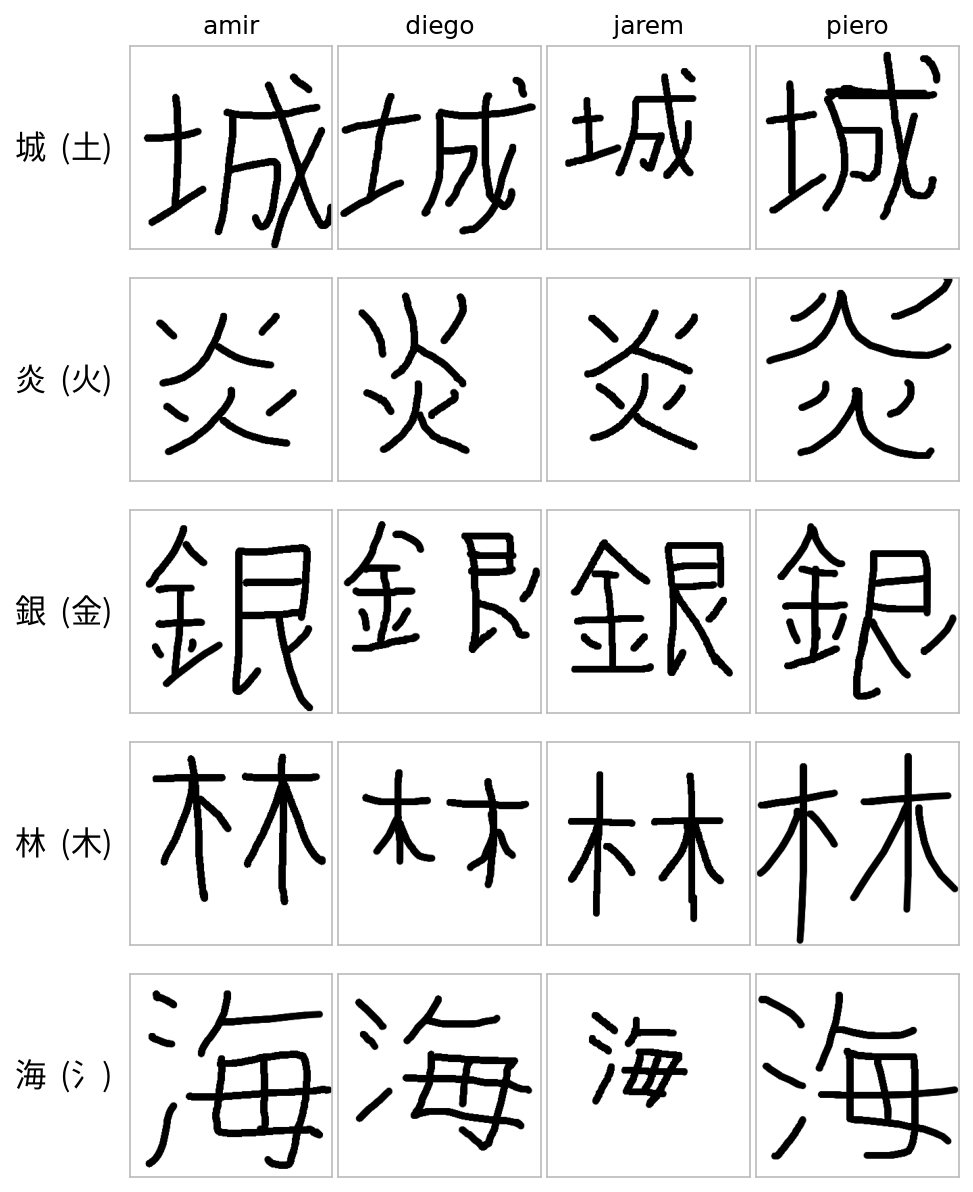
\includegraphics[height=0.76\textheight]{figures/writers_grid.png}
    \end{column}
    \begin{column}{0.48\textwidth}
      \small
      Un kanji por radical (3.ª repetición de cada escritor).

      \medskip
      Cambian de un escritor a otro:
      \begin{itemize}
        \item tamaño y posición en el lienzo,
        \item proporciones entre radical y resto,
        \item inclinación y forma de cada trazo.
      \end{itemize}

      \medskip
      El preprocesado elimina lo primero; lo demás lo tiene que aprender la red.
    \end{column}
  \end{columns}
\end{frame}

\begin{frame}{Dataset}
  \centering
  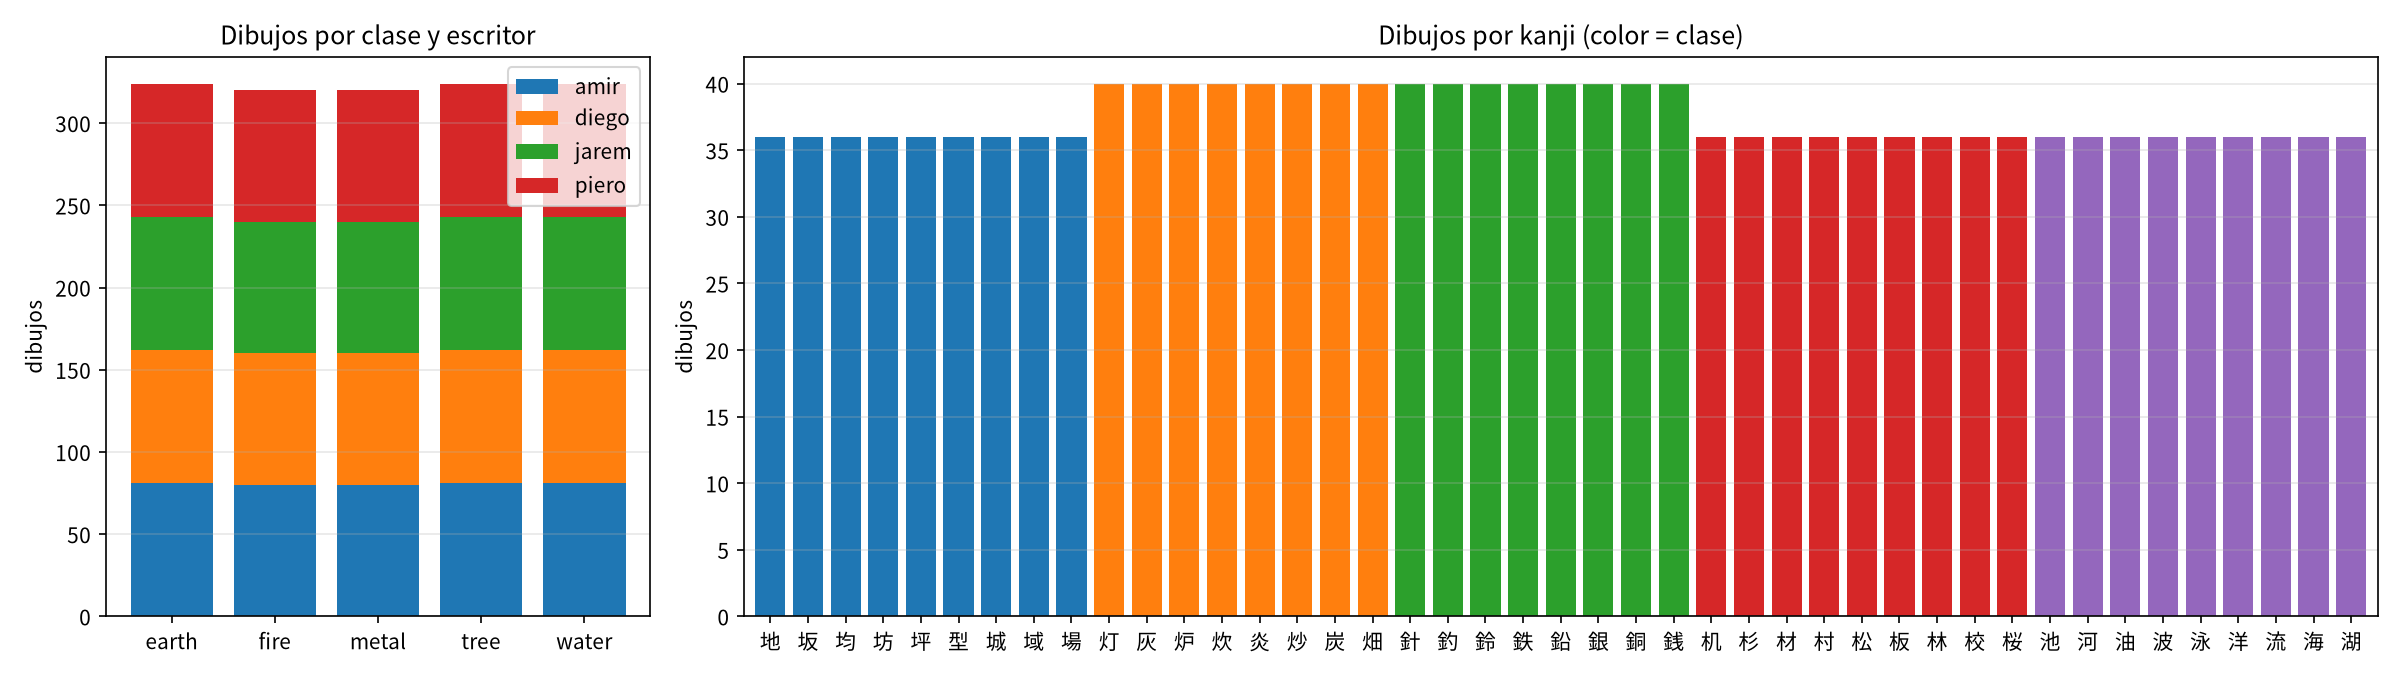
\includegraphics[width=0.92\textwidth]{figures/dataset_counts.png}

  \smallskip
  \begin{tabular}{cccc}
    \textbf{1612} dibujos & \textbf{403} por escritor & \textbf{320–324} por radical & \textbf{36–40} por kanji
  \end{tabular}
\end{frame}

% ---------------------------------------------------------------------------
\section{Preprocesado y aumento de datos}

\begin{frame}{Preprocesado}
  \centering
  \begin{tikzpicture}[
      stage/.style={draw=mDarkTeal, fill=soft, rounded corners=3pt, align=center,
                   minimum height=1.5cm, text width=2.1cm, font=\small},
      arr/.style={-{Stealth[length=6pt]}, thick, mDarkTeal}]
    \node[stage] (a) {PNG RGBA\\300×300};
    \node[stage, right=0.45cm of a] (b) {canal alfa\\tinta = 1};
    \node[stage, right=0.45cm of b] (c) {recorte a la caja del kanji};
    \node[stage, right=0.45cm of c] (d) {cuadrado con 8\,\% de margen};
    \node[stage, right=0.45cm of d] (e) {64×64\\LANCZOS};
    \foreach \x/\y in {a/b, b/c, c/d, d/e} \draw[arr] (\x) -- (\y);
  \end{tikzpicture}

  \bigskip
  \begin{itemize}
    \item El recorte y el centrado quitan el efecto de \textbf{dónde y a qué tamaño} se dibujó, pero el padding cuadrado \textbf{no deforma} el kanji: se conserva dónde está el radical (izquierda, abajo…).
    \item A 64×64 el pincel de 10\,px queda en unos \textbf{2\,px}.
    \item Salida: tensor $1\times64\times64$ en $[0,1]$. Los 1612 dibujos se cargan en memoria (unos 26\,MB).
    \item Manifiesto \texttt{data/build/drawings\_index.csv}: ruta, etiqueta, kanji, escritor y split de cada dibujo.
  \end{itemize}
\end{frame}

\begin{frame}{División train / val / test}
  \begin{columns}[T]
    \begin{column}{0.5\textwidth}
      \textbf{70 / 15 / 15}, \textbf{estratificado por kanji}: cada kanji (y cada radical) aparece en los tres conjuntos en la misma proporción.

      \medskip
      {\small
      \begin{tabular}{lrl}
        \toprule
        Conjunto & Dibujos & Uso \\
        \midrule
        train & 1128 & ajuste de pesos \\
        val   & 242  & LR y mejor época \\
        test  & 242  & solo métricas finales \\
        \bottomrule
      \end{tabular}}

      \medskip
      \small Semilla 42. Cada corrida guarda una \textbf{huella} (sha1 de las rutas): si cambian los dibujos, no se mezclan corridas.
    \end{column}
    \begin{column}{0.46\textwidth}
    \end{column}
  \end{columns}
\end{frame}

\begin{frame}{Aumento de datos: 4 transformaciones}
  \textbf{Solo en train}, sobre la imagen ya preprocesada (64×64). Cada dibujo genera una variante de cada tipo:

  \smallskip
  \centering
  \small
  \renewcommand{\arraystretch}{1.2}
  \begin{tabular}{lll}
    \toprule
    Transformación & Qué hace & Parámetro \\
    \midrule
    ruido gaussiano & suma $\mathcal{N}(0,\sigma)$ a cada píxel & $\sigma \in [0.05, 0.15]$ \\
    sal y pimienta + media & $p$ de los píxeles a 0 o 1; media 3×3 & $p \in [0.02, 0.06]$ \\
    sal y pimienta + mediana & el mismo ruido; mediana 3×3 & $p \in [0.02, 0.06]$ \\
    rotación & giro alrededor del centro & $\pm 3^\circ$ a $\pm 15^\circ$ \\
    \bottomrule
  \end{tabular}

  \raggedright
  \medskip
  \footnotesize
  \begin{itemize}
    \item Sobre el PNG de 300×300, el ruido repartido por el lienzo arruinaría el recorte a la caja del kanji.
    \item Filtros de 3×3: con trazos de unos 2\,px, uno de 5×5 los borraría.
    \item Sin volteos: cambiarían el lado del radical (\jp{氵} siempre va a la izquierda).
  \end{itemize}
\end{frame}

\begin{frame}{Ejemplos del aumento}
  \begin{columns}[c]
    \begin{column}{0.56\textwidth}
      \centering
      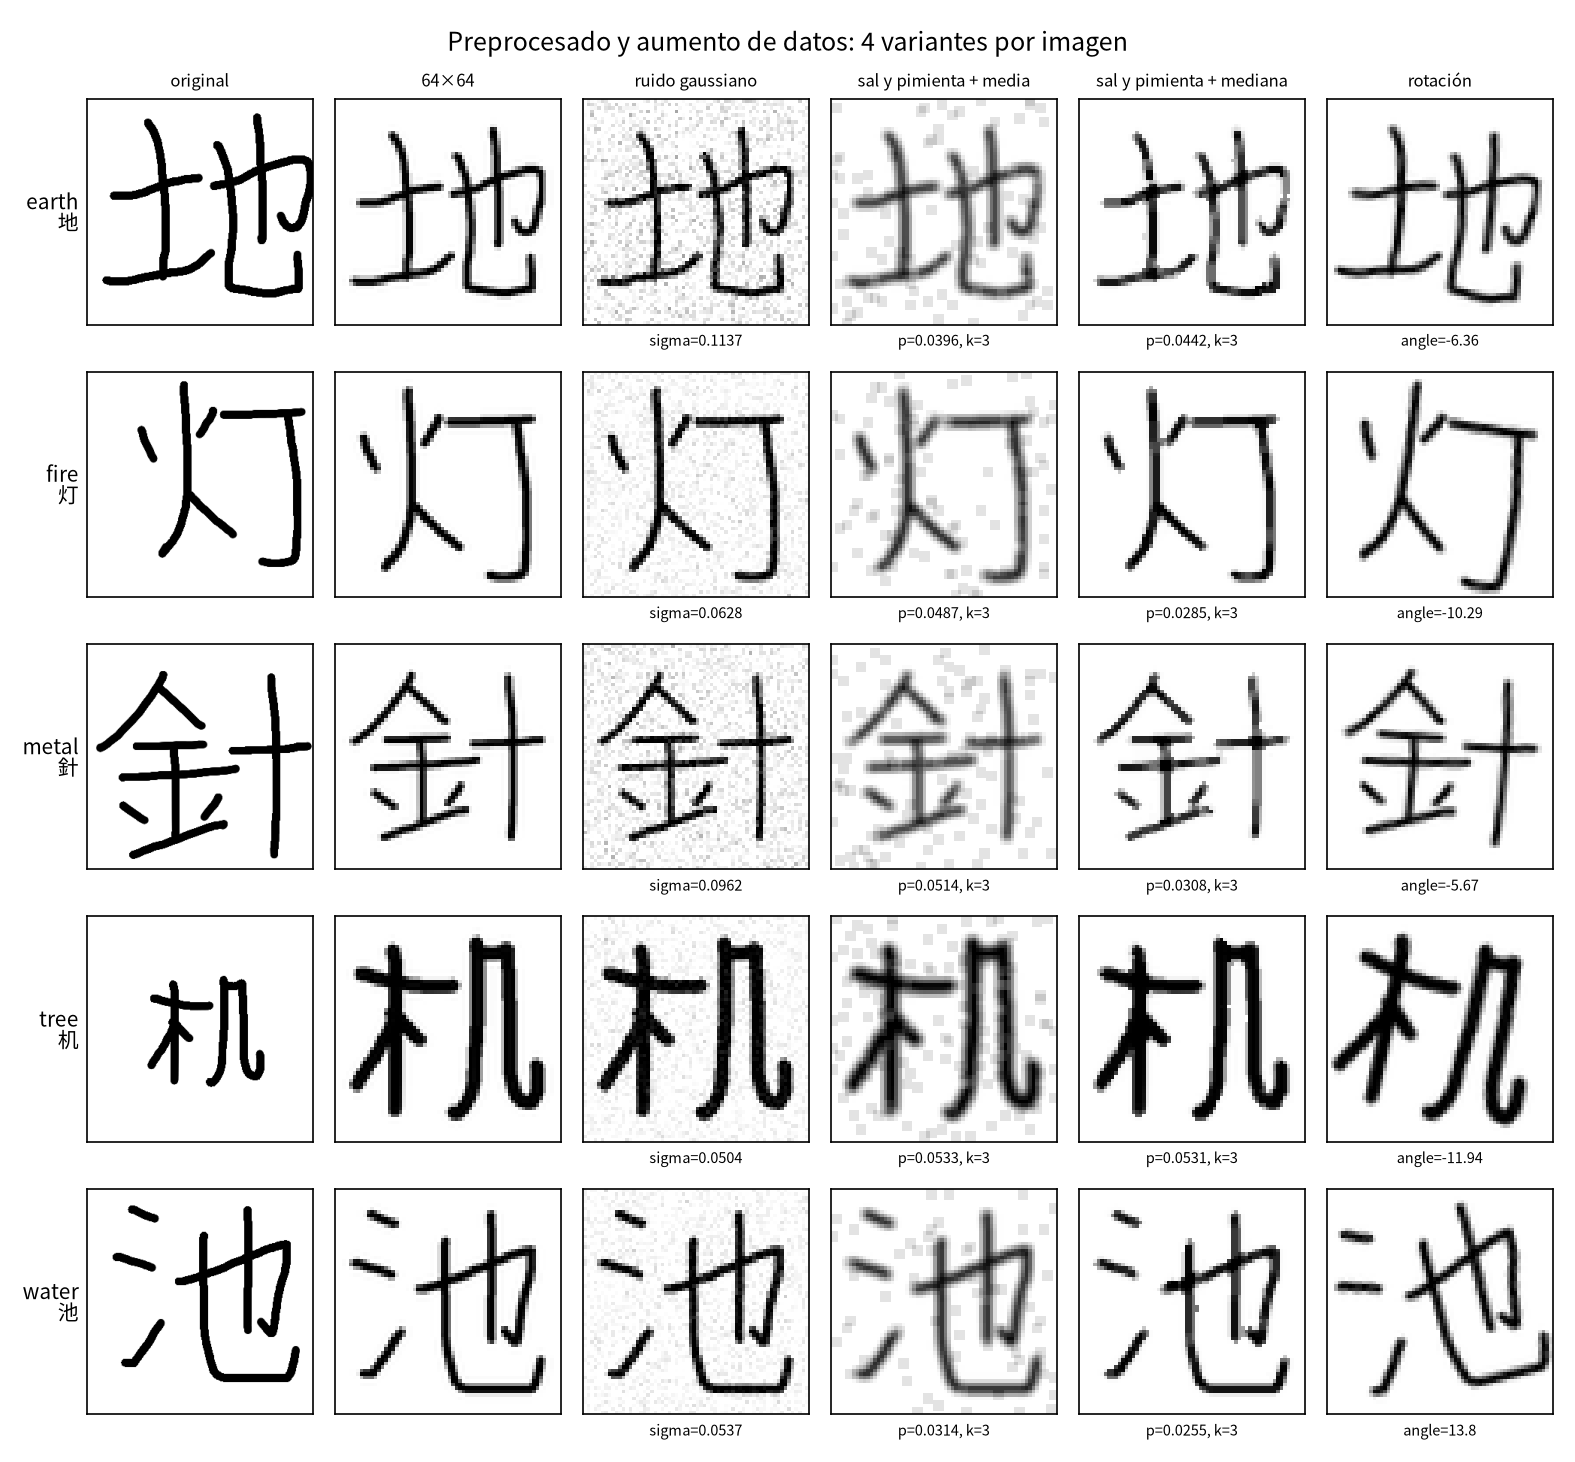
\includegraphics[height=0.76\textheight]{figures/augmentation.png}
    \end{column}
    \begin{column}{0.42\textwidth}
      Un dibujo por radical: original $\to$ 64×64 $\to$ sus 4 variantes, con sus parámetros.

      \bigskip
      \begin{itemize}
        \item La \textbf{mediana} elimina casi todo el ruido impulsivo sin difuminar el trazo.
        \item La \textbf{media} lo difumina, pero no lo quita.
        \item La rotación no recorta el kanji gracias al margen del 8\,\%.
      \end{itemize}
    \end{column}
  \end{columns}
\end{frame}

\begin{frame}{Cuántas imágenes: entre 500 y 1000 por radical}
  Objetivo común para todas las clases, con $n_c$ = originales de train del radical $c$:
  \[
    T = \min\bigl(\max(5 \cdot \textstyle\max_c n_c,\ 500),\ 1000\bigr)
  \]
  \vspace{-0.6em}
  \begin{columns}[c]
    \begin{column}{0.38\textwidth}
      \small
      \begin{itemize}
        \item $n_c \approx 227$: $5 \cdot 227 = 1135 > 1000$, así que $T = \mathbf{1000}$.
        \item Train: \textbf{5000 imágenes}, clases iguales.
        \item Cada original queda con 3 o 4 variantes.
        \item Registro: \texttt{train\_augmented.csv}.
      \end{itemize}
    \end{column}
    \begin{column}{0.6\textwidth}
      \centering
      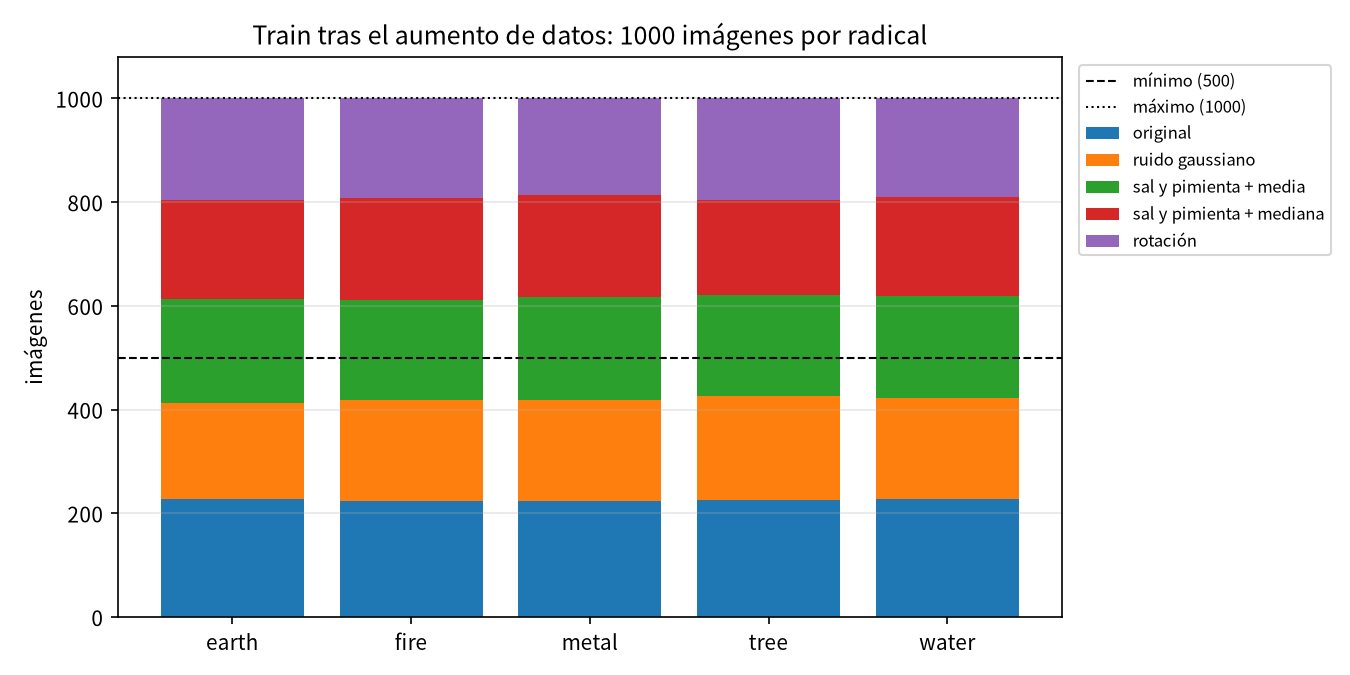
\includegraphics[width=\textwidth]{figures/augmentation_counts.png}
    \end{column}
  \end{columns}
\end{frame}

% ---------------------------------------------------------------------------
\section{Modelos y entrenamiento}

\begin{frame}{Nuestra CNN: \texttt{KanjiRadicalCNN}}
  \centering
  \begin{tikzpicture}[
      blk/.style={draw=mDarkTeal, fill=mDarkTeal!12, rounded corners=2pt, align=center,
                  minimum height=1.6cm, text width=1.3cm, inner sep=2pt, font=\footnotesize},
      head/.style={blk, fill=mLightBrown!20, draw=mLightBrown},
      arr/.style={-{Stealth[length=5pt]}, thick, black!60}]
    \node[blk, fill=white] (in) {entrada\\1×64×64};
    \node[blk, right=0.25cm of in] (b1) {bloque\\32 canales\\{\scriptsize 32×32}};
    \node[blk, right=0.25cm of b1] (b2) {bloque\\64 canales\\{\scriptsize 16×16}};
    \node[blk, right=0.25cm of b2] (b3) {bloque\\128 canales\\{\scriptsize 8×8}};
    \node[blk, right=0.25cm of b3] (b4) {bloque\\256 canales\\{\scriptsize 4×4}};
    \node[head, right=0.25cm of b4] (gap) {global avg pool\\256};
    \node[head, right=0.25cm of gap] (fc1) {FC 256\\ReLU\\Dropout 0.4};
    \node[head, right=0.25cm of fc1] (fc2) {FC 5\\softmax};
    \foreach \x/\y in {in/b1, b1/b2, b2/b3, b3/b4, b4/gap, gap/fc1, fc1/fc2} \draw[arr] (\x) -- (\y);
  \end{tikzpicture}

  \bigskip
  \begin{columns}[T]
    \begin{column}{0.5\textwidth}
      \begin{block}{Cada bloque}
        \small $[\text{Conv } 3{\times}3 \to \text{BatchNorm} \to \text{ReLU}] \times 2 \to \text{MaxPool } 2{\times}2$
      \end{block}
    \end{column}
    \begin{column}{0.44\textwidth}
      \begin{itemize}
        \item \textbf{1.24\,M} parámetros (4.7\,MB).
        \item El \emph{global average pooling} evita una capa densa enorme sobre el mapa de 4×4.
      \end{itemize}
    \end{column}
  \end{columns}
\end{frame}

\begin{frame}{La referencia: ResNet50 preentrenada en ImageNet}
  \begin{columns}[T]
    \begin{column}{0.55\textwidth}
      \begin{itemize}
        \item \texttt{torchvision} con pesos \texttt{IMAGENET1K\_V2}; se ajustan \textbf{todas} las capas.
        \item \textbf{1 canal}: los pesos RGB de \texttt{conv1} se suman. Da la misma respuesta que la convolución original sobre la imagen gris replicada en los 3 canales.
        \item Normalización gris equivalente a ImageNet: media 0.449, desviación 0.226.
        \item \texttt{fc}: 2048 $\to$ 5.
      \end{itemize}
    \end{column}
    \begin{column}{0.4\textwidth}
      \begin{block}{¿Por qué compararla?}
        \small Con un dataset pequeño, el \emph{transfer learning} desde ImageNet es lo que suele recomendarse. Si la CNN propia la iguala, una red 19 veces más pequeña basta.
      \end{block}
      \medskip
      \centering
      \begin{tabular}{lr}
        \toprule
        parámetros & 23.5\,M \\
        tamaño     & 89.9\,MB \\
        \bottomrule
      \end{tabular}
    \end{column}
  \end{columns}
\end{frame}

\begin{frame}{Entrenamiento}
  \centering
  \small
  \renewcommand{\arraystretch}{1.3}
  \begin{tabular}{ll}
    \toprule
    optimizador & Adam \\
    learning rate inicial & $10^{-3}$ (CNN) \quad $10^{-4}$ (ResNet50, ya preentrenada) \\
    pérdida & cross-entropy con \emph{label smoothing} 0.1 \\
    scheduler & \texttt{ReduceLROnPlateau} sobre \texttt{val\_loss} (factor 0.5, paciencia 3) \\
    épocas y batch & 20 épocas, batches de 32 (5000 imágenes por época) \\
    modelo final & pesos de la época con menor \texttt{val\_loss} \\
    \bottomrule
  \end{tabular}

  \bigskip
  \raggedright
  Las dos redes usan \textbf{el mismo split, el mismo train aumentado y el mismo test}: la huella del dataset se comprueba antes de comparar.
\end{frame}

% ---------------------------------------------------------------------------
\section{Resultados}

\begin{frame}{CNN: curvas de entrenamiento}
  \centering
  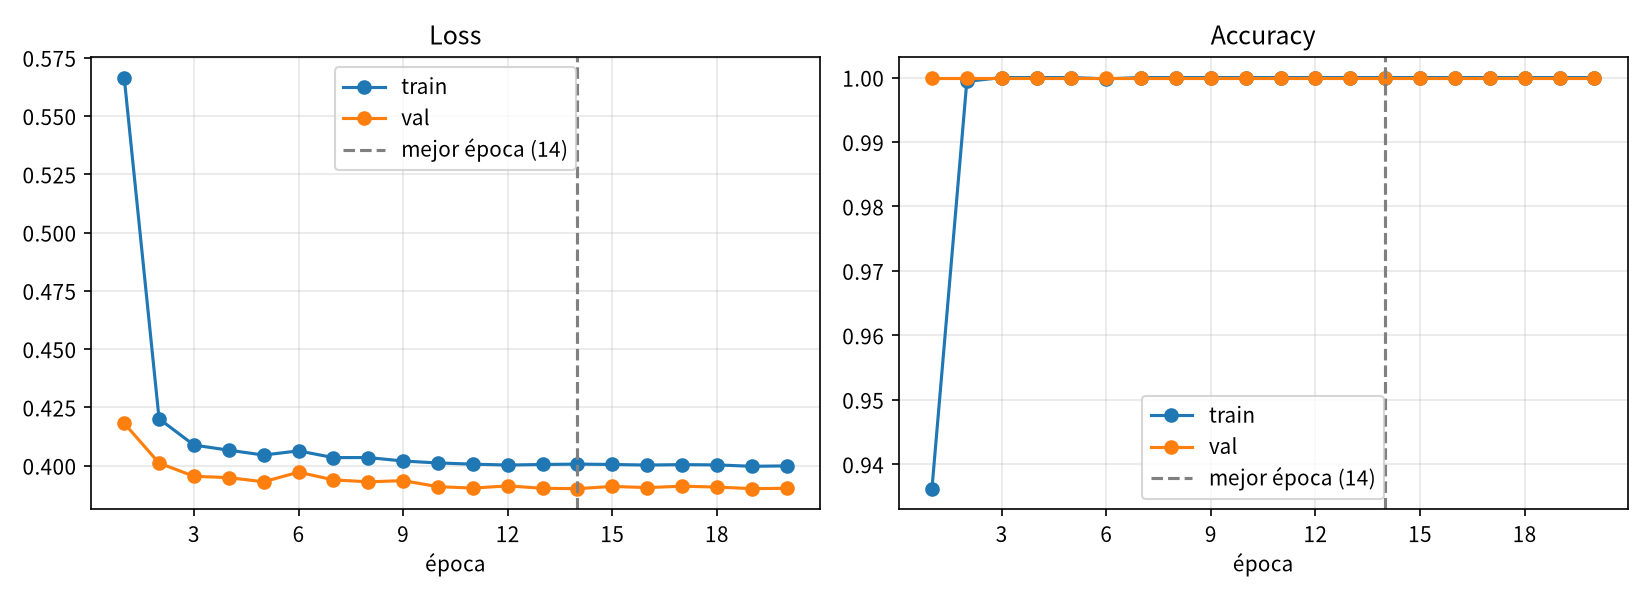
\includegraphics[width=0.94\textwidth]{figures/cnn_curves.png}

  \raggedright
  \begin{itemize}
    \item Val acc = 1 desde la primera época; la pérdida sigue bajando hasta la \textbf{época 14} (menor \texttt{val\_loss}).
    \item La pérdida no baja de $\approx 0.39$ por el \emph{label smoothing}. Unos 35\,s por época en CPU.
  \end{itemize}
\end{frame}

\begin{frame}{CNN: test (242 dibujos)}
  \begin{columns}[c]
    \begin{column}{0.44\textwidth}
      \centering
      \renewcommand{\arraystretch}{1.25}
      \begin{tabular}{lr}
        \toprule
        Métrica & CNN \\
        \midrule
        accuracy            & 1.000 \\
        precision (macro)   & 1.000 \\
        recall (macro)      & 1.000 \\
        F1 (macro)          & 1.000 \\
        loss                & 0.390 \\
        inferencia          & 2.5\,ms/img \\
        \bottomrule
      \end{tabular}

      \bigskip
      \raggedright
      \small Acierta los 242 dibujos de test, de los 43 kanji y los 4 escritores.
    \end{column}
    \begin{column}{0.54\textwidth}
      \centering
      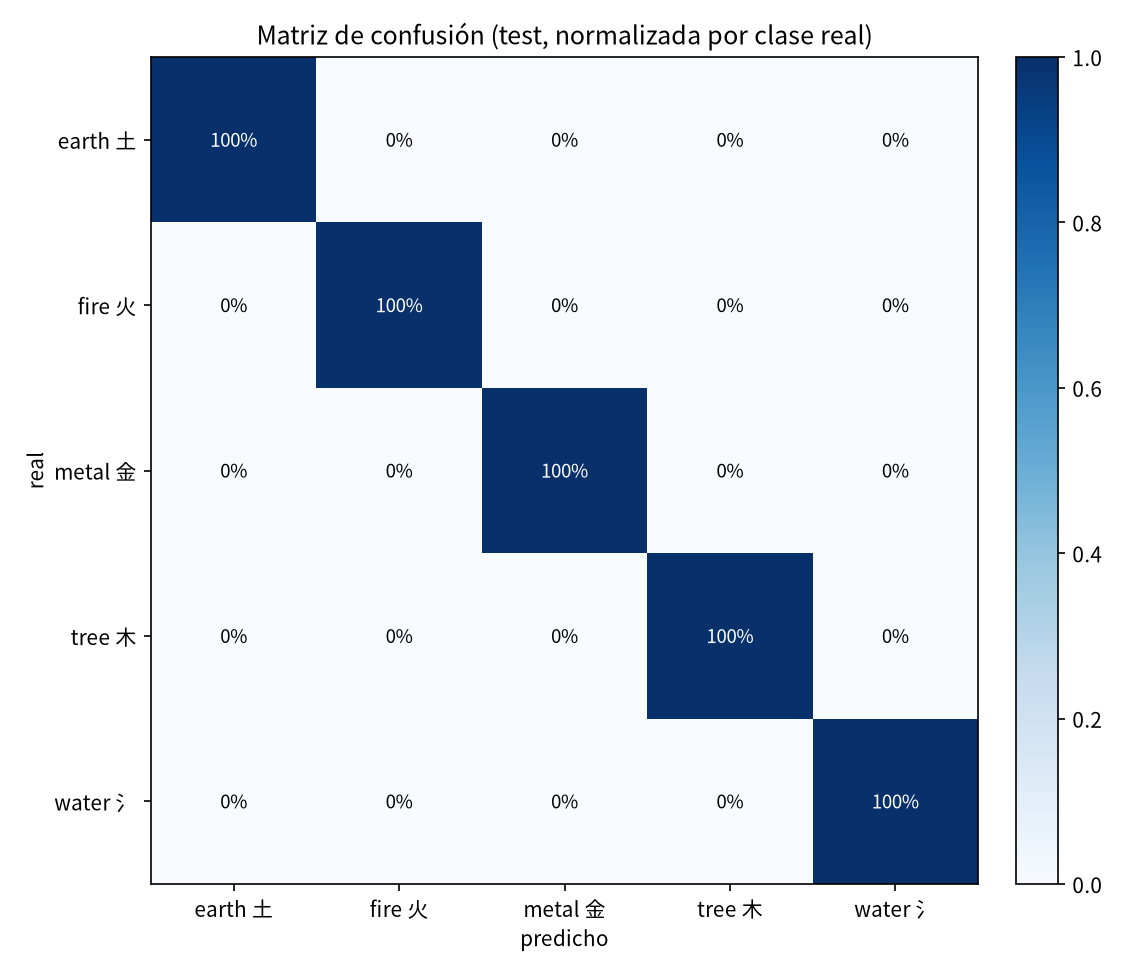
\includegraphics[height=0.8\textheight]{figures/cnn_confusion_matrix.png}
    \end{column}
  \end{columns}
\end{frame}

\begin{frame}{Cómo se compara con la ResNet50}
  \texttt{make train-resnet compare} (o \texttt{kanji-compare runs/cnn runs/resnet50}):

  \small
  \begin{itemize}
    \item Comprueba que las dos corridas usan los mismos dibujos, clases, semilla y test.
    \item \textbf{Métricas de test} con intervalo de confianza del 95\,\% (\emph{bootstrap}, 1000 remuestreos).
    \item \textbf{Test de McNemar exacto}: compara solo los dibujos en que una red acierta y la otra falla. Dos redes con la misma accuracy pueden fallar en imágenes distintas.
    \item \textbf{Coste}: parámetros, tamaño, segundos por época y milisegundos por imagen.
    \item Figuras: métricas, curvas superpuestas, diferencia de F1 por radical y dibujos en que discrepan.
  \end{itemize}

  \medskip
  Salida en \texttt{data/runs/compare/}: \texttt{comparison.json}, \texttt{comparison.md} y figuras.
\end{frame}

\begin{frame}{Comparación: resultados}
  \begin{columns}[T]
    \begin{column}{0.55\textwidth}
      \textbf{Precisión en test}

      \smallskip
      \small
      \begin{tabular}{lcc}
        \toprule
        Corrida & CNN & ResNet50 \\
        \midrule
        Preliminar: 484 dibujos, & \multirow{2}{*}{1.000} & \multirow{2}{*}{1.000} \\[-2pt]
        \quad sin aumento, test $n=73$ & & \\
        Completa: 1612 dibujos, & \multirow{2}{*}{1.000} & \multirow{2}{*}{\emph{pendiente}} \\[-2pt]
        \quad con aumento, test $n=242$ & & \\
        \bottomrule
      \end{tabular}

      \medskip
      Preliminar: McNemar $p = 1$ (ningún dibujo en que discrepen).
    \end{column}
    \begin{column}{0.42\textwidth}
      \textbf{Coste}

      \smallskip
      \small
      \begin{tabular}{lrr}
        \toprule
         & CNN & ResNet50 \\
        \midrule
        parámetros   & 1.24\,M & 23.5\,M \\
        tamaño       & 4.7\,MB & 89.9\,MB \\
        s/época$^{*}$ & 5 & 9 \\
        ms/img$^{*}$  & 3.8 & 4.7 \\
        \bottomrule
      \end{tabular}

      \smallskip
      \scriptsize $^{*}$ Corrida preliminar, en CPU.
    \end{column}
  \end{columns}

  \bigskip
  \begin{exampleblock}{Lectura}
    \small Con este split las dos redes aciertan todo: no hay diferencia de precisión que medir, solo de coste. La CNN propia es \textbf{19 veces más pequeña}.
  \end{exampleblock}
\end{frame}

% ---------------------------------------------------------------------------
\section{Conclusiones}

\begin{frame}{Limitaciones y trabajo futuro}
  \begin{itemize}
    \item \textbf{El test aleatorio es demasiado fácil}: comparte kanji y escritor con train. Un 100\,\% no separa a las dos redes.
    \item \textbf{Split por escritor}: dejar a un escritor entero en test (el manifiesto guarda el escritor de cada dibujo). Mediría la generalización a letra nueva.
    \item \textbf{Split por kanji}: dejar kanji enteros fuera de train. Mediría si la red reconoce el radical en kanji que nunca vio.
    \item \textbf{Más escritores}: con 4 personas, la variedad de letra es limitada.
    \item Con T = 1000, no caben las 4 variantes de cada dibujo: o se sube el máximo, o se usan menos originales.
  \end{itemize}
\end{frame}

\begin{frame}[fragile]{Reproducibilidad}
  \begin{columns}[T]
    \begin{column}{0.53\textwidth}
      \begin{block}{Comandos}
\footnotesize
\begin{verbatim}
make draw          # app de dibujo
make dataset       # manifiestos y aumento
make train         # CNN
make train-resnet  # ResNet50
make compare       # CNN vs ResNet50
make notebooks     # local y Colab
\end{verbatim}
      \end{block}
    \end{column}
    \begin{column}{0.44\textwidth}
      \small
      \begin{itemize}
        \item Cada corrida guarda en \texttt{data/runs/} \texttt{model.pt}, \texttt{history.json}, \texttt{metrics.json}, \texttt{predictions.npz} y sus figuras.
        \item Notebooks \textbf{local} y \textbf{Colab} (datos en Drive) con el mismo flujo: mismo split y mismo train aumentado que la línea de comandos.
        \item El split y el aumento son deterministas con \texttt{-{}-seed} (42 por defecto).
      \end{itemize}
    \end{column}
  \end{columns}
\end{frame}

\begin{frame}{Conclusiones}
  \begin{itemize}
    \item Construimos el flujo completo: \textbf{dibujo $\to$ etiquetado $\to$ preprocesado $\to$ aumento $\to$ entrenamiento $\to$ evaluación $\to$ comparación}.
    \item El aumento de datos lleva train a \textbf{1000 imágenes por radical}, con las clases equilibradas, sin tocar val ni test.
    \item Nuestra CNN de \textbf{1.24\,M parámetros} acierta el 100\,\% del test (242 dibujos).
    \item Frente a la ResNet50, en la corrida preliminar empatan en precisión, con una red 19 veces más pequeña.
    \item El siguiente paso es un \textbf{test más exigente} (por escritor o por kanji) para medir de verdad la generalización.
  \end{itemize}
\end{frame}

\begin{frame}[standout]
  ¿Preguntas?

  \bigskip
  \jp{\Huge 土　火　金　木　氵}
\end{frame}

\end{document}
